\section{Graphisches Modell}\label{sec:graphischesmodell}
Im vorherigen Kapitel wurde das grundlegende Programmierungskonzept von flowws erklärt und anhand der Anforderungen gegenüber dem System sowie anhand der Probleme bestehender Systeme begründet. Wie allerdings schon in der Einleitung (Kapitel \ref{sec:einleitungkonzept}) geschrieben, benötigt die \ac{EUD} eine graphische Oberfläche, mit welcher der Endnutzer interagieren kann. Auch hier werden Entscheidungen anhand von Anforderungen, Probleme und \textit{Best-Practice-Frameworks} wie \ac{CD} rationalisiert.
 
\subsection{Design Richtlinien}
Für die graphische Oberfläche von flowws müssen die einzelnen Elemente, die im vorherigen Kapitel beschrieben wurden durch eine graphischen Repräsentant abgebildet werden. Der Endnutzer muss mit diesen Abbildungen interagieren, um die gewünschte Betriebsverhalten des Gesamtsystems zu erreichen. Um eine kohärente \ac{UX} zu erreichen, sollen Abbildung und Interaktion einer geteilten Philosophie unterliegen; einem Satz von Regeln, der die Design-Entscheidungen rationalisiert und sich an den Rahmenbedingungen des Projekts orientiert.

\paragraph{Nähe zur Realität} Es sollte immer bedacht werden, dass die (physischen) cBlocks zu jedem Zeitpunkt des Design Prozesses verwendet werden. Graphisch soll diese physische Bindung reflektiert werden. Aus diesem Grund soll die visuelle Darstellung und die Interaktionen der \ac{EUD} wenn möglich Bezug zu den cBlocks oder zumindest mit der Domäne der \ac{IoT} und Elektrotechnik besitzen. Es wird sich dadurch erhofft, dass \textbf{Domänennähe} und \textbf{funktionale Aussagekraft} (siehe Tabelle \ref{tab:cognitivedimensions}) zu erhöhen und somit die Anforderungen NFN\#2 und NFN\#3 zu lösen.

\paragraph{Fokus bewahren} Design ist ein kreativer Prozess von dem flowws nicht durch seine eigene Komplexität bzgl. des Prototypingprozess ablenken soll. Um schnell und zielführend Arbeiten zu können, soll flowws Vorgaben machen an denen sich der Endnutzer orientieren kann. Durch graphische Signale wie Farben und Formen soll dem Nutzer das Rätseln über die Rolle einzelner Komponenten erspart werden.

\paragraph{Fehler vorbeugen} Statt zeitaufwändige Fehlersuche zu unterstützen ist es sinnvoller Fehler durch graphische Hinweise im Vorfeld zu vermeiden (siehe Tabelle \ref{tab:cognitivedimensions} und NFN\#4).

\paragraph{''Move fast and break things''} Prototyping ist schnell und explorativ. Deswegen soll die \ac{GUI} von flowws diese schnelle Art von Arbeit durch bspw. Austauschbarkeit der Komponenten unterstützen.

\paragraph{''Grow-As-You-Go''} flowws ist kein Lehrwerkzeug sondern soll produktives Arbeiten ermöglichen. Die technischen Fähigkeiten der Endnutzer sind allerdings sehr Variabel. Zusätzlich ist zu erwarten, dass das technische Verständnis mit der stetigen Benutzung des Werkzeugs wächst. Daher soll der Funktionsumfang der Oberfläche mit den Fähigkeiten des Endnutzers wachsen können. Das Erlernen der Oberfläche durch nützliche Hinweise unterstützen (NFN\#2). Gleichzeitig aber soll sie nicht obsolet werden, bei komplexeren Szenarien, in denen spezifischere Funktionalität abverlangt wird (NFN\#5).

%%%%%%%%%%%%%%%%%%%%%%%%%%%%%%%%%%%%%%%%%%%%%%%%%%%%%%%%%%%%%%%%%%%%%%%%%%%%%%%%%%%%%%%%%%%%%%%%%%%%%%%%%%%%%%%%%%%%%%%%%%

\subsection{Workspace}
\begin{figure}[h]
  \centering
  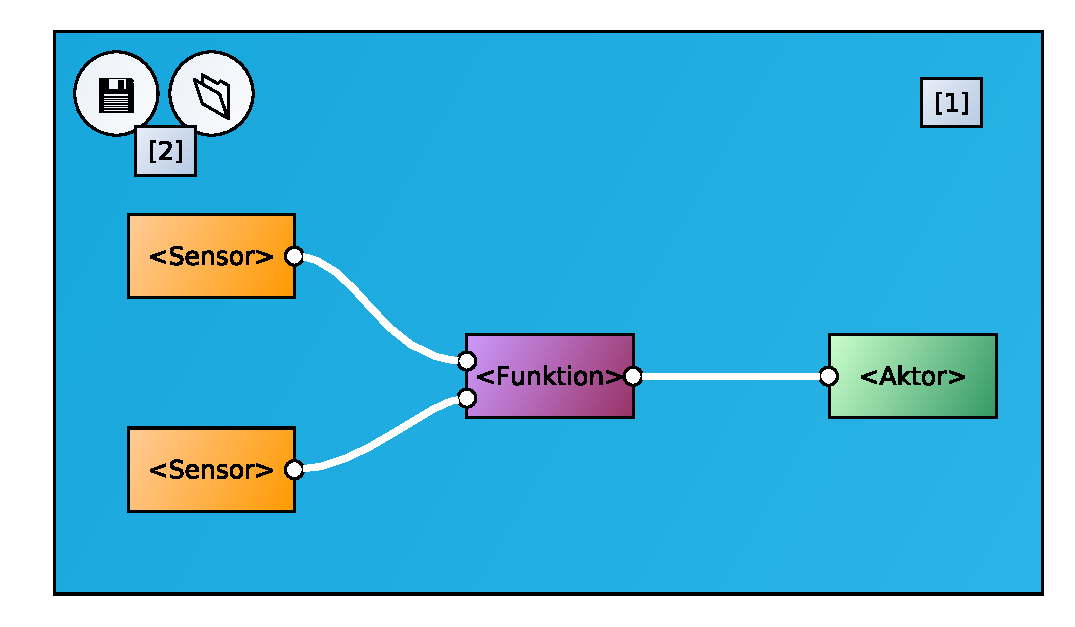
\includegraphics[width=.75\textwidth]{bilder/chapter4/chapter4_3/workspace.pdf}
  \caption{[1] ist der Workspace mit einem generischen Graph. [2] erlauben die Graphen zu manipulieren.}
  \label{fig:genericlink}
\end{figure}


\paragraph{Kurzbeschreibung} Der Workspace (engl. Arbeitsbereich) ist die primäre Komponente von flowws. Innerhalb dieser Komponente werden flowws-Graphen bzw. flowws-Programme erstellt, organisiert, administriert und auf Fehler untersucht. Er dient als digitale Leinwand für den Designer, um im Zusammenspiel mit den physischen cBlocks Prototypen zu erstellen.

\paragraph{Rahmenbedingungen \& Entscheidungen} Aufgrund der Gegebenheiten der cBlocks, arbeitet der Endnutzer zu jederzeit an nur einem Graphen. Dies steht im Kontrast zur Programmierung in \acp{IDE}, in denen an mehreren Projekten simultan gearbeitet werden kann und somit ein hoher Grad von Kontextwechsel benötigt wird. Bei flowws soll sich der Designer ähnlich wie bei einer Leinwand vollständig auf die Erstellung des Graphen konzentrieren können, ohne sich mit einer Kakophonie von Icons und Untermenüs auseinandersetzen zu müssen. flowws wird immer simultan zu cBlocks verwendet, d.h. der Endnutzer manipuliert und interagiert während des gesamten Entwicklungszyklus mit den cBlocks

Die \textbf{Aufgaben}, die in dieser Komponente durchgeführt werden gehört: 
\begin{itemize}
    \item \textbf{Anzeigen von Knoten} Der Workspace dient dem Anzeigen von Sensor- und Aktorknoten. 
    \item \textbf{Administration von Graphen} Der Graph kann über den Workspace gespeichert, geladen und verwaltet werden. 
\end{itemize}

\paragraph{Darstellung} Der Workspace ist wie in Abbildung [ref] gezeigt, spartanisch gehalten. Bis auf zwei Knöpfe zum Laden und Speichern von Graphen sind keine weiteren Interaktionsmöglichkeiten zu sehen. Diese Entscheidung wurde bewusst so getroffen. Der leere Workspace soll einen leeren Schreibtisch nachahmen (''Nähe zur Realität''). Aus diesem Grund, werden Sensorknoten und Aktorknoten automatisch angezeigt, wenn ihre physischen Gegenstücke mit dem System verbunden sind. Die Schreibtisch-Metapher soll durch ein optisches Anlehnen der Oberfläche an eine typische Schneideunterlage weiter unterstützt werden.

%%%%%%%%%%%%%%%%%%%%%%%%%%%%%%%%%%%%%%%%%%%%%%%%%%%%%%%%%%%%%%%%%%%%%%%%%%%%%%%%%%%%%%%%%%%%%%%%%%%%%%%%%%%%%%%%%%%%%%%%%%
\subsubsection{flowws-Graph}
\subsubsection{Knoten}
\begin{figure}[h]
  \centering
  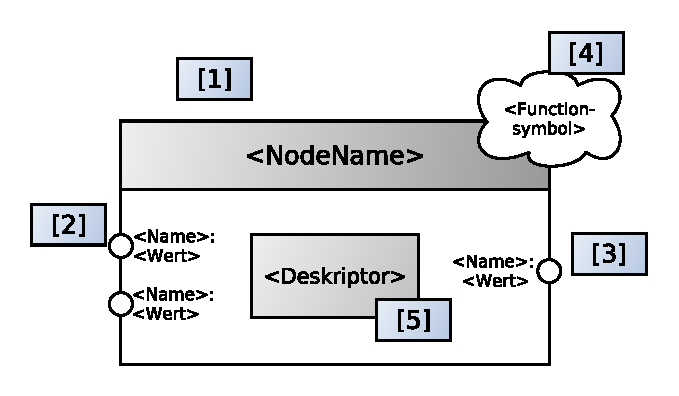
\includegraphics[width=.75\textwidth]{bilder/chapter4/chapter4_3/genericnode.pdf}
  \caption{Ein generischer Knoten.}
  \label{fig:genericnode}
\end{figure}

\paragraph{Kurzbeschreibung} Knoten sind die fundamentalen Bausteine eines jeden flowws-Graphen. Sie erzeugen, transformieren und konsumieren Daten auf die Weise, auf die sie vom Endnutzer kompositioniert sind. Alle Knoten (Sensoren, Funktionen, Aktoren) teilen fundamentale Charakteristiken (Identität, Form), Subkomponenten (Input-/Output-Schnittstellen, Deskriptor) und Interaktionen (Anordnen, Erstellen, Löschen) miteinander. 

\paragraph{Rahmenbedingungen \& Entscheidungen} Ein jeder Block muss eindeutig von seinem Typus identifizierbar und seinem physischen Pendant zuordenbar sein. Da es viele Sorten von Knoten gibt, muss es möglichst leicht erkenntlich sein, welche Funktion er übernimmt, welche Daten ein- und ausfließen und aus welchem Grund der Block seine Entscheidung getroffen hat.

Der Endnutzer kann folgende \textbf{Operationen} in dieser Komponente durchführen: 
\begin{itemize}
    \item \textbf{Anordnen} Die Knoten lassen sich hinsichtlich ihrer Position organisieren bzw. anordnen. Dadurch kann der Endnutzer die Position der physischen Aktoren/Sensoren mit denen der Virtuellen abgleichen (siehe ''Nähe zur Realität'').
    \item \textbf{Verbindung starten/enden} Die Schnittstellen dienen als Interaktionspunkte um Verbindungen zu starten und zu enden.
    \item \textbf{Deskriptor ändern} Durch das ändern des Deskriptors kann das Verhalten von Knoten auf Eingangssignale modifiziert werden.
\end{itemize}

\paragraph{Darstellung} Der in Abbildung \ref{fig:genericnode} dargestellte generische Block besitzt alle Merkmale, die in Aktor-,Sensor- und Funktionsknoten vorhanden sind. Die quadratische Darstellung des Knoten wurde einer komplexeren Darstellung bevorzugt, um eine visuelle Nähe zum Quader-Design der cBlocks zu erreichen (siehe Abbildung [abb cBlocks]). \textbf{[1]} ist die Identifikationsleiste des Blocks. Sie gibt durch Farbe Aufschluss über den Typ (\colorbox{sensororange}{Sensor}, \colorbox{aktorgreen}{Aktor} und \colorbox{funcviolet}{Funktion}) und durch Text Aufschluss über die Rolle (z.B. ''Logisches-Gatter'') des Knotens. \textbf{[2]} und \textbf{[3]} sind die Input- und Output Schnittstellen. Sie dienen als Anfangs- und Endpunkte für Verbindungen, besitzen Namen durch die sie Unterscheidbar werden (''OperandA'' etc.) und zeigen den letzten Wert an, der über die Schnittstelle empfangen bzw. versendet wurde (siehe NFN\#1). \textbf{[4]} ist der Knoten-Indikator und gibt wie \textbf{[2]} Aufschluss über den Knotentyp und Knotenrolle. Er zeigt zum einen durch seine Form den Typ und zum Anderen mit einem Symbol die konkrete Rolle des Knotens (bspw. Temperatur-Sensor, Funktionsknoten: Logisches-Gatter, etc.) an. \textbf{[5]} ist der Knoten-Deskriptor. Er gibt Endnutzer Aufschluss, welche konkrete Instruktion (bspw. logisches Und) auf den Eingabedaten ausgeführt werden bzw. in welchem Zustand sich der Knoten momentan befindet.

%%%%%%%%%%%%%%%%%%%%%%%%%%%%%%%%%%%%%%%%%%%%%%%%%%%%%%%%%%%%%%%%%%%%%%%%%%%%%%%%%%%%%%%%%%%%%%%%%%%%%%%%%%%%%%%%%%%%%%%%%%

\subsubsection{Verbindungen/Kanten}
\begin{figure}[h]
  \centering
  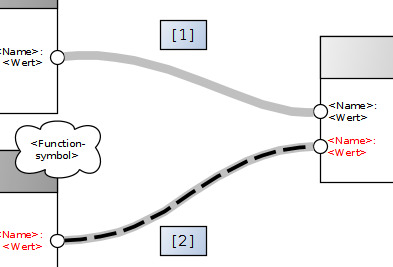
\includegraphics[width=.55\textwidth]{bilder/chapter4/chapter4_3/links.png}
  \caption{Zwei Kanten verbinden vier Input-/Output-Schnittstellen. [1] ist inaktiv während über [2] ein Signal übertragen wird. Man beachte die kurzzeitige Färbung der Input-/Output-Schnittstellen, die auf eine Aktualisierung des Wertes hinweisen.}
  \label{fig:genericlink}
\end{figure}


\paragraph{Kurzbeschreibung} Verbindungen/Kanten sind die Transportwege der Daten, zwischen den einzelnen Knoten. Ähnlich wie ein Kabel auf einer Platine stellen eine Kante den Transportweg der Signale von einer Output-Schnittstelle zu einer Input-Schnittstelle dar.

\paragraph{Rahmenbedingungen \& Entscheidungen} Jede Verbindung stellt eine eins-zu-eins Beziehung zwischen zwei Schnittstellen dar. Dabei muss sichergestellt werden, das nur Schnittstellen mit kompatiblen Datentypen verbunden werden können (NFN\#4). 

Der Endnutzer kann folgende \textbf{Operationen} in dieser Komponente durchführen: 
\begin{itemize}
    \item \textbf{Erstellen} Durch betätigen einer Output-Schnittstelle wird der Erstellungprozess einer Verbindung gestartet und endet mit dem Betätigen einer kompatiblen Input-Schnittstelle oder dem Erstellen eines kompatiblen Funktionsknotens.
    \item \textbf{Löschen} Löscht die Datenübertragung zwischen zwei Schnittstellen und bereinigt die Input-Schnittstelle, in der die Verbindung versinkt.
\end{itemize}

\paragraph{Darstellung} Die Darstellung einer Verbindung ist eine Bézierkurve, die an einer Input-Schnittstelle entsteht und an einer Output-Schnittstelle endet (Abbildung \ref{fig:genericlink}). Sobald Daten durch eine Verbindung fließen, wird eine kurze Animation innerhalb der Bézierkurve gespielt, die den Transfer von Daten entlang der Flußrichtung darstellt ([2]). Der Datentransfer geht verzögerungsfrei von Statten, ähnlich wie der Transfer von elektrischen Signalen durch Kabel. Deswegen wird die Animation über die ganze Länge der Kurve kurzlebig dargestellt (siehe ''Nähe zur Realität'').

%%%%%%%%%%%%%%%%%%%%%%%%%%%%%%%%%%%%%%%%%%%%%%%%%%%%%%%%%%%%%%%%%%%%%%%%%%%%%%%%%%%%%%%%%%%%%%%%%%%%%%%%%%%%%%%%%%%%%%%%%%

\subsubsection{Sensorknoten}
\begin{figure}[h]
\centering
\begin{subfigure}{.5\textwidth}
  \centering
  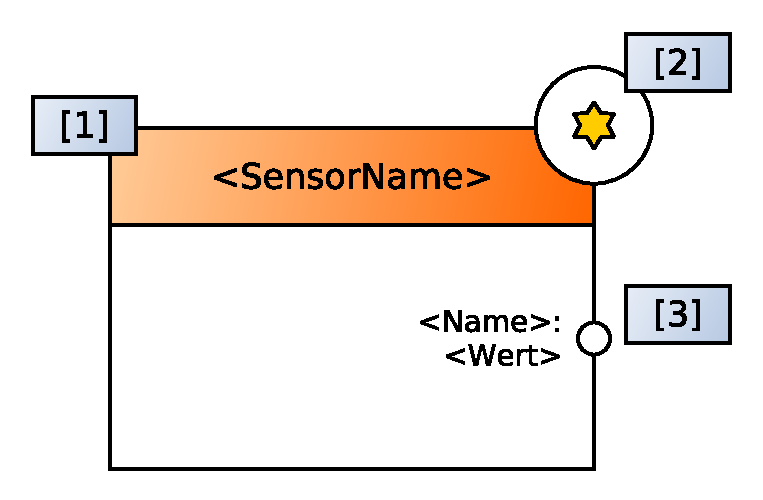
\includegraphics[width=1\linewidth]{bilder/chapter4/chapter4_3/genericsensornode.pdf}
  \caption{}
  \label{fig:genericsensornode}
\end{subfigure}%
\begin{subfigure}{.5\textwidth}
  \centering
  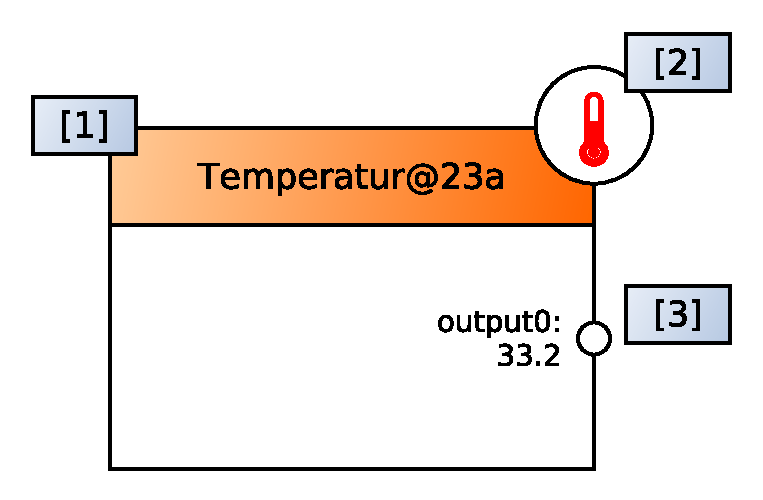
\includegraphics[width=1\linewidth]{bilder/chapter4/chapter4_3/instancesensornode.pdf}
  \caption{}
  \label{fig:sensornodetemperature}
\end{subfigure}
    \caption{Generischer Sensorknoten (a) und Temperatur-Sensorknoten (b)}
    \label{fig:sensornodes}
\end{figure}

\paragraph{Kurzbeschreibung}  Sensorknoten sind die virtuellen Gegenstücke zu den Sensor-cBlocks. Jeder Sensorknoten erzeugt Ereignisse, sobald der Sensor-cBlock eine neue Stichprobe in der Realität entnimmt. Alle Ereignisse werden mit einem Datentyp und dem Messwert als \textit{Payload} über die Output-Schnittstelle an nachfolgende Knoten verteilt. Sobald ein Sensorknoten angezeigt wird sendet er stetig Daten und erlaubt dem Endnutzer kontinuierlich das Verhalten des Graphen zu überprüfen (siehe ''Fehler vorbeugen'').

\paragraph{Rahmenbedingungen \& Entscheidungen} Einzelne Sensor-cBlocks können mehrere verschiedene Messwerte auslesen (bspw. Temperatur und Luftfeuchtigkeit im selben Sensor-cBlock). Der Sensorknoten muss es möglich sein, diese Multimodalität abbilden zu können. Es kann sein, dass mehrere Sensor-cBlocks von der gleichen Sorte im selben Prototypen verwendet werden. In diesem Fall muss es für den Endnutzer möglich sein die Sensorknoten klar unterscheiden zu können. Gleichzeitig muss es dem Nutzer möglich sein leicht das  physikalische Pendant zu einem virtuellen Sensorknoten zu identifizieren. Ein weiterer Punkt ist die Abtastfrequenz. Sensor-cBlocks liefern Daten in kurz-, lang- oder aperiodischen Frequenzen . Sensorknoten müssen aus diesem Grund darauf achten, synchron mit ihrem physischen Gegenstück, Ereignisse zu erzeugen. Sensorknoten können weder erstellt noch gelöscht werden. Der Status des Sensorknotens, also auch seine Existenz, ist an dem Status des Sensor-cBlocks gebunden.

Der Endnutzer kann folgende \textbf{Operationen} in dieser Komponente durchführen: 
\begin{itemize}
    \item \textbf{Identifizieren} durch Betätigen des Knoten-Indikators blinkt die Status LED des korrespondierenden cBlocks. Somit lässt sich sein physisches Pendant identifizieren.
\end{itemize}
\paragraph{Darstellung} In Abbildung \ref{fig:sensornodes} ist ein generischer Sensorknoten (a) und ein konkreter Temperatur-Sensorknoten (b) dargestellt. Jeder Sensorknoten ist durch eine eindeutige Adresse in der Titelleiste [1] voneinander unterscheidbar. Simultan wird durch \textbf{[2]} der Blocktyp ($\bigcirc$) und seine Rolle (Thermometer = Temperatur) preisgegeben. \textbf{[3]} sind die Output-Schnittstellen. Jede Art von Messwert eines Sensor-cBlocks erhält einen separaten Output, der die aktuellsten Messwert visualisiert. 

%%%%%%%%%%%%%%%%%%%%%%%%%%%%%%%%%%%%%%%%%%%%%%%%%%%%%%%%%%%%%%%%%%%%%%%%%%%%%%%%%%%%%%%%%%%%%%%%%%%%%%%%%%%%%%%%%%%%%%%%%%

\subsubsection{Funktionsknoten}
\begin{figure}[h]
\centering
\begin{subfigure}{.5\textwidth}
  \centering
  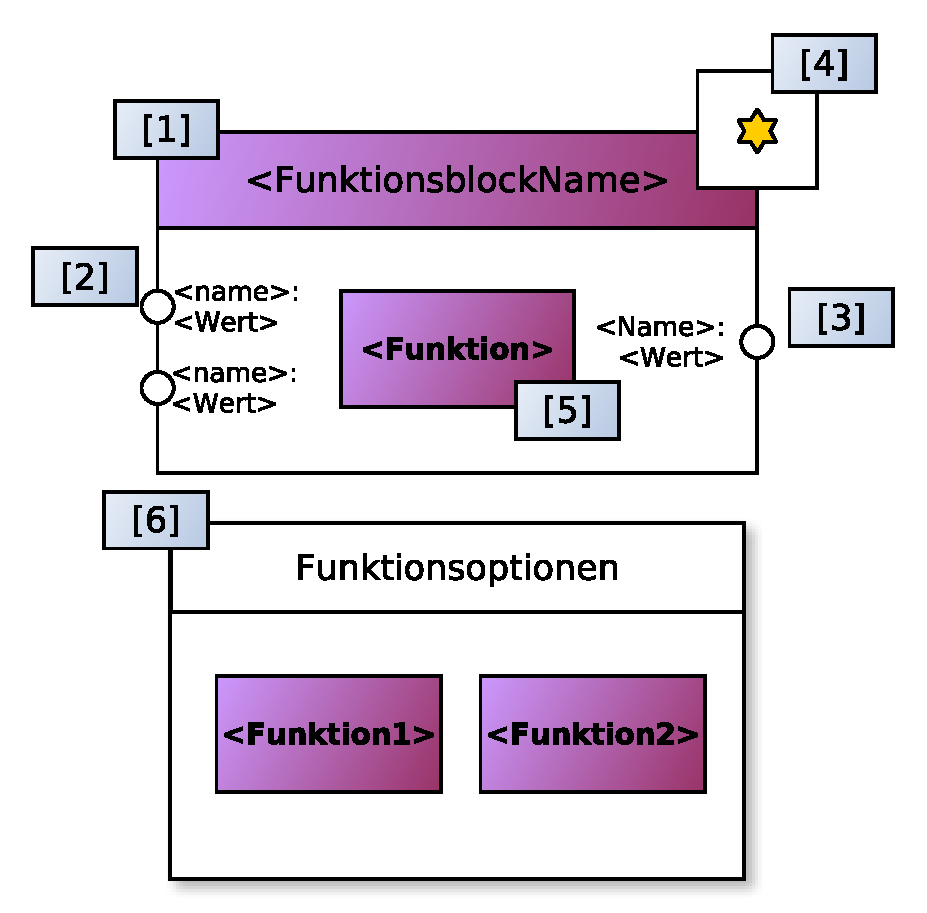
\includegraphics[width=1\linewidth]{bilder/chapter4/chapter4_3/genericfunctionnode.pdf}
  \caption{}
  \label{fig:functionnodesgen}
\end{subfigure}%
\begin{subfigure}{.5\textwidth}
  \centering
  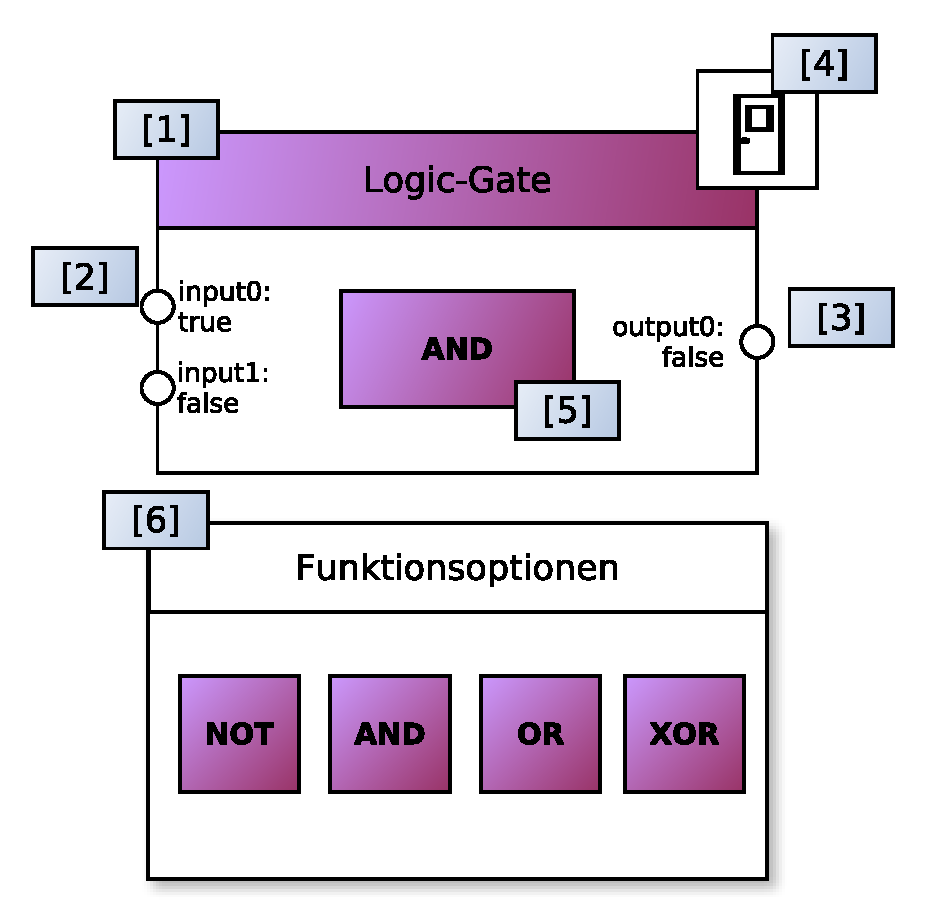
\includegraphics[width=1\linewidth]{bilder/chapter4/chapter4_3/instancegatefunctionnode.pdf}
  \caption{}
  \label{fig:functionnodesgate}
\end{subfigure}
    \caption{Generischer Funktionsknoten (a) und spezifischer Funktionsknoten ''Logisches-Gatter'' (b). Weitere Beispiele für Funktionsknoten im Anhang \ref{anhang:funktionsknoten}}
    \label{fig:functionnodes}
\end{figure}

\paragraph{Kurzbeschreibung} Funktionsknoten sind die Rechnereinheiten des Graphen. Der Endnutzer benutzt sie um Signale zu kombinieren und aufzuwerten. Funktionsknoten kommen in einer Bandbreite von Operationsklassen (Logisches-Gatter, Vergleichsoperation, etc.), welche sich an den Datentypen der Ereignisse orientieren (\texttt{String}, \texttt{Number} und \texttt{Boolean}). Jede Operationsart besitzt eine Familie von entsprechenden Operatoren ($\neg, \land,\neq,\geq,$ etc.).

\paragraph{Rahmenbedingungen \& Entscheidungen} Es wurde sich dafür entschieden, Operatoren in Operationsklassen zu bündeln, statt jeder Operation in einen separaten Funktionsknoten auszulagern. Dies soll der Übersicht beitragen und somit das Prototyping beschleunigen (siehe ''Move fast...''). Des Weiteren lässt sich dadurch die Funktion austauschen ohne den Block und somit die Verbindungen austauschen zu müssen (siehe ''vorzeitige Festlegung'' in Tabelle \ref{tab:cognitivedimensions}). Dies beschleunigt das Experimentieren mit verschiedenen Operatoren. Funktionsknoten sind rein virtuell und generisch, sprich anders als bei Sensoren/Aktoren können zwei komplett identische Knoten im gleichen Graph existieren.

Der Endnutzer kann folgende \textbf{Operationen} in dieser Komponente durchführen: 
\begin{itemize}
    \item \textbf{Löschen} Funktionsknoten begründen ihre Existenz nicht auf ein physisches Pendant, deshalb sind sie anders als Sensor-/Aktorknoten löschbar.
    \item \textbf{Konfigurieren} Die konkrete Funktion muss durch Interagieren mit dem Deskriptor gewählt werden (siehe Abbildung \ref{functionnodes} und Anhang \ref{anhang:funktionsknoten} für weitere Beispiele)
\end{itemize}

\paragraph{Darstellung}  Der Deskriptor [5] ermöglicht es den momentanen Operator auszulesen. Durch betätigen von [5] wird ein \textit{Modal} geöffnet, indem sich der Operator konfigurieren lässt. In Abbildung \ref{fig:functionnodesgate} ist als Beispiel ein Logikgatter-Funktionsknoten dargestellt. Hier kann der Nutzer die verschiedenen bool'schen Operatoren im laufenden Betrieb ändern, und somit das Verhalten des gesamten Graphen zu Laufzeit ändern (siehe '' Immiidiate feedback''). Die Schnittstellen [2] und [3] erlauben Parameter und Ergebnis zur Laufzeit auszulesen und Fehler zu überprüfen.

%%%%%%%%%%%%%%%%%%%%%%%%%%%%%%%%%%%%%%%%%%%%%%%%%%%%%%%%%%%%%%%%%%%%%%%%%%%%%%%%%%%%%%%%%%%%%%%%%%%%%%%%%%%%%%%%%%%%%%%%%%

\subsubsection{Aktorknoten}

\begin{figure}[h]
\centering
\begin{subfigure}{.55\textwidth}
  \centering
  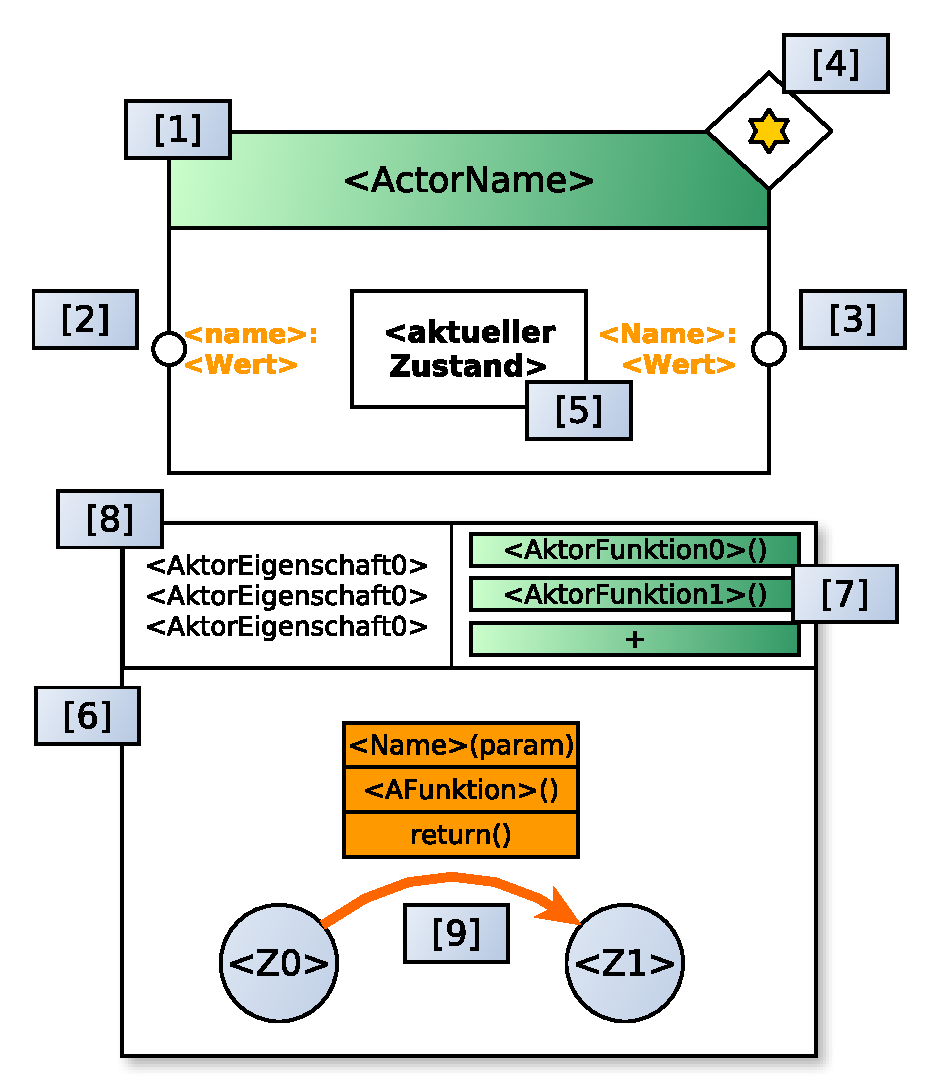
\includegraphics[width=1\linewidth]{bilder/chapter4/chapter4_3/genericactornode.pdf}
  \caption{}
  \label{fig:actorgeneric}
\end{subfigure}%
\begin{subfigure}{.55\textwidth}
  \centering
  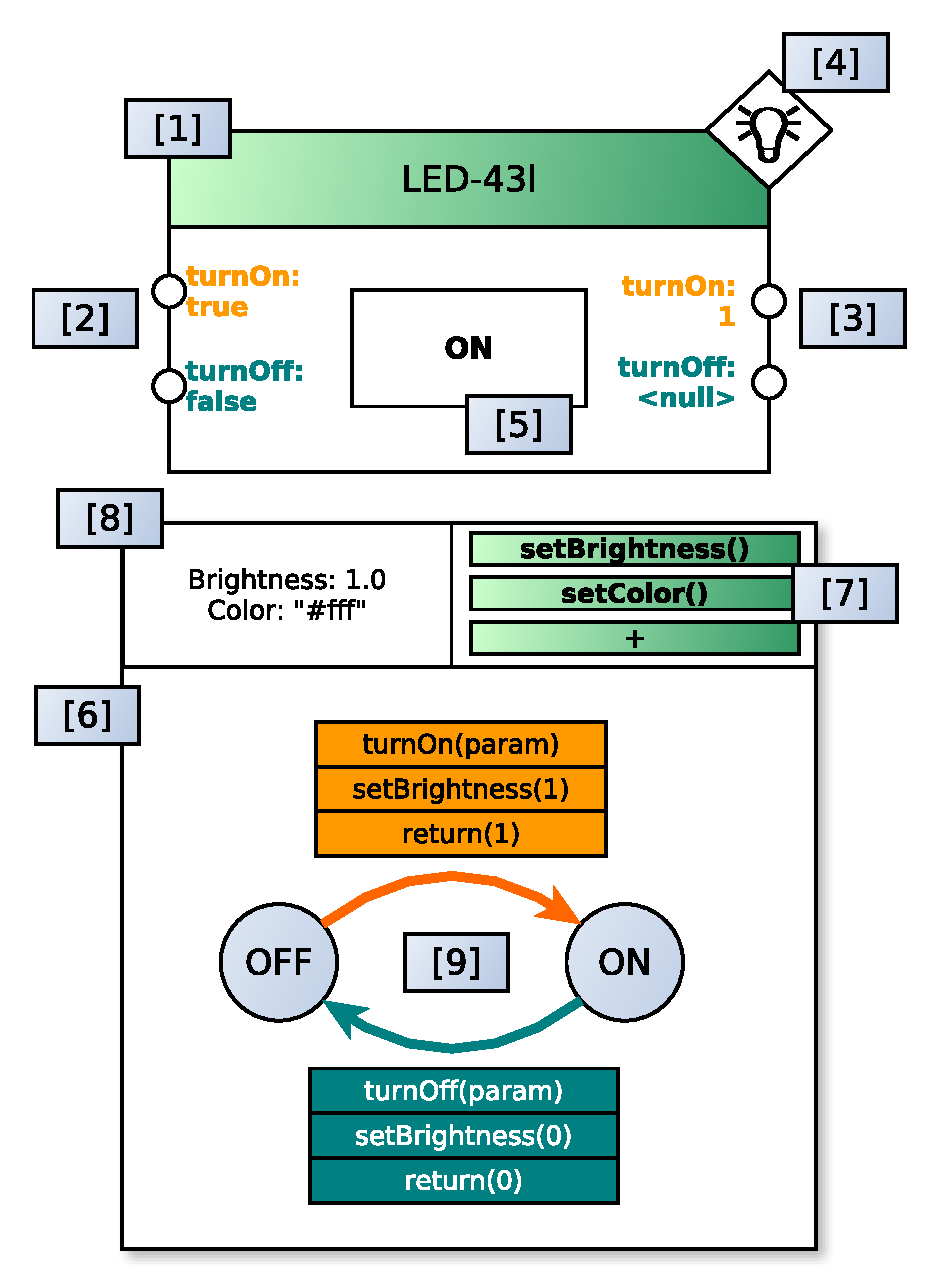
\includegraphics[width=1\linewidth]{bilder/chapter4/chapter4_3/instanceLEDactornode.pdf}
  \caption{}
  \label{fig:actorled}
\end{subfigure}
    \caption{Generischer Aktorblock (a) und spezifischer LED-Aktorblock (b)}
    \label{fig:actornodes}
\end{figure}


\paragraph{Kurzbeschreibung} Aktorknoten sind Sensorknoten sehr ähnlich. Auch ihr Zustand ist an den des Aktor-cBlocks gebunden (siehe ''Nähe zur Realität''). Jeder Aktorknoten besitzt eine \ac{FSM}, die vom Endnutzer modelliert wird. Diese \ac{FSM} (siehe Abbildung \ref{fig:actorled} [6]) erlaubt es durch Aktorfunktionen (bspw. \texttt{setColor()}), Aktoreigenschaften (bspw. \texttt{color}) zu verändern und somit die physikalischen Signale des Aktor-cBlocks zu manipulieren.

\paragraph{Rahmenbedingungen \& Entscheidungen} Aktorknoten sind neben dem eigentlichen Graphen die zweite programmierbare Komponente in flowws. Jeder Aktorknoten besitzt eine eingeschränkte Menge von Eigenschaften, die direkt mit den physikalischen Eigenschaften des Aktor-cBlocks korrespondieren. Ein Minimum von Aktorfunktionen wird von flowws vorgegeben. Des Weiteren kann der Endnutzern die Aktorfunktionen jedes Aktorknotens nach belieben erweitern (siehe ''Grow as you go''). Nutzern soll es gleichzeitig möglich sein, mit den selben Gesten, mit denen der Graph modelliert wird, auch die \ac{FSM} zu programmieren (siehe ''Fokus bewahren''). Dem Nutzer soll zu jedem Zeitpunkt möglich sein das Verhalten des Aktors vorauszusagen und nachvollziehen zu können. Aktoren sollen ihren Zustand dem Rest des Graphen mitteilen zu können. Deshalb soll es der Endnutzer in der Lage sein, synthetische Signale zu definieren, die bei einem Zustandswechsel erzeugt werden.

Der Endnutzer kann folgende \textbf{Operationen} in dieser Komponente durchführen: 
\begin{itemize}
    \item \textbf{\ac{FSM} erstellen} Zustände, Übergänge und Übergangsfunktionen werden mithilfe der Aktorfunktionen und Aktoreigenschaften vom Endnutzer modelliert
    \item \textbf{Umfang der Aktorfunktionen erweitern} Um den Funktionsumfang zu erweitern können zustandslose Funktionen, welche Aktoreigenschaften modifizieren, vom Endnutzer in Programmcode spezifiziert werden.
\end{itemize}

\paragraph{Darstellung} Der Aktorknoten wird ähnlich wie der Funktionsknoten auf zwei Ebenen dargestellt: der Graphen-Ebene [1] und in Detail-Ebene [8]. Input- [2] und Output-Schnittstellen [3] korrespondieren bei Aktorknoten farblich und namentlich mit den Zustandsübergängen [9] um die Sichtbarkeit des Verhaltens auch außerhalb der Detailansicht zu garantieren (siehe ''Sichtbarkeit'' in Tabelle \ref{tab:cognitivedimensions}). Die momentane Ausprägung der Aktoreigenschaften wird in [8] dargestellt. Die verfügbaren Aktorfunktionen sind in [7] inspizierbar. Die Darstellung der \ac{FSM} in [9] orientiert sich am ist simpel gehalten mit Kreisen, die Zustände symbolisieren und farbigen Pfeilen, die Übergänge definieren. Die Überganglogik wird in einer dreigeteilten Box dargestellt, die sich in Deklaration (Name korrespondiert mit [2] und [3]), Logik (Aktorfunktionen) und Rückgabewert (Der \textit{Payload} des vom Aktor erzeugten Events) aufteilt. Zur Laufzeit ist der momentane Zustand des Aktorknotens ist im Deskriptor [5] ersichtlich.

\subsubsection{Radialmenü}

\begin{figure}[h]
  \centering
  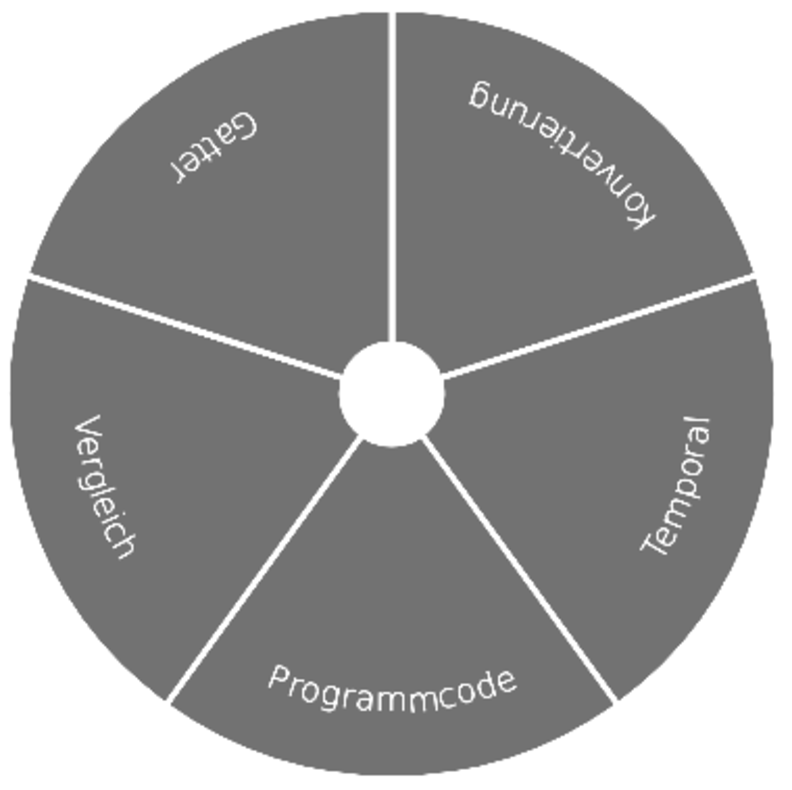
\includegraphics[width=.4\textwidth]{bilder/chapter4/chapter4_3/radialmenu.pdf}
  \caption{Das Radialmenu mit den fünf verschiedenen Operationsklassen aus Kapitel \ref{subsubsec:eventtrans} zur Auswahl}
  \label{fig:radialmenu}
\end{figure}

\paragraph{Kurzbeschreibung} Das Radialmenü ist ein Untermenü, das zu jeder Zeit auf dem Workspace aufgerufen werden kann. Es wird vom Endnutzer verwendet, um Funktionsknoten zu erzeugen.

\paragraph{Rahmenbedingungen \& Entscheidungen} Es wurde sich für ein Radialmenü entschieden, da es im Vergleich zu linearen Menüs schneller zu benutzen ist (siehe ''Move fast...'). Vor allem bei einer vergleichsweise geringen Anzahl von Optionen, die oft verwendet werden müssen (was bei flowws der Fall ist) sind laut \cite{kurtenbach1994user} Radialmenüs besonders effektiv. Das Menü ist kontextsensitiv, d.h. es zeigt immer nur Operationsklassen von Funktionsknoten an die zu diesem Zeitpunkt relevant sind. Dies soll zum einen, die Auswahl von inkompatiblen Funktionsknoten verhindern (siehe ''Fehler vorbeugen'') und zum anderen, durch das Verstecken unnötiger Informationen die Arbeitsgeschwindigkeit erhöhen (siehe ''Move fast...'').

Der Endnutzer kann folgende \textbf{Operationen} in dieser Komponente durchführen: 
\begin{itemize}
    \item \textbf{Funktionsknoten erstellen} Das Radialmenü ist der einzige Weg für den Nutzer Funktionsknoten zu erstellen. Dazu ruft der Endnutzer das Radialmenü auf und wählt den gewünschten Funktionsknoten aus.
\end{itemize}

\paragraph{Darstellung} Das Radialmenü (Abbildung \ref{fig:radialmenu}) ist in fünf Segmente aufgeteilt, bei dem jedes Segment eine Art von Funktionsknoten repräsentiert. Das Radialmenü wird nur nach explizitem Aufruf durch den Endnutzer oder im Kontext von Interaktionen dargestellt und ist sonst nicht sichtbar. 

\subsection{Interaktionen}

Gibt nur wenige Interaktionen. Beschränkt sich hier auf das wichtigste. Meisten Interaktionen sind Drag-and-Drop basiert, um die nähe zur Realität zu behalten (da cBlocks ja auch in ihrer Position manipuliert werden können).

\subsubsection{Verbinden von Knoten}

\begin{figure}[h]
  \centering
  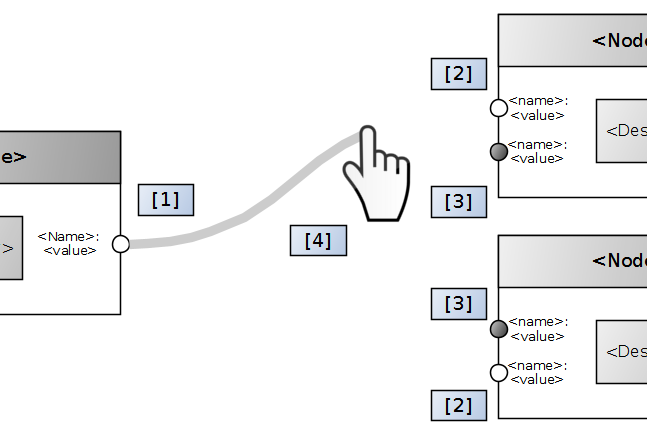
\includegraphics[width=.75\textwidth]{bilder/chapter4/chapter4_3/connectNodes.png}
  \caption{Das Radialmenu mit den fünf verschiedenen Operationsklassen aus Kapitel \ref{subsubsec:eventtrans} zur Auswahl}
  \label{fig:connectNodesInteraction}
\end{figure}
Das Modellieren des Graphen in flowws ist äquivalent mit dem Programmieren von Programmcode. Neben dem Modellieren von \ac{FSM} um das Verhalten von Aktoren zu steuern ist die Hauptarbeit in flowws das Verbinden von Knoten. Das Verbinden von Knoten soll an das Verbinden von Hardware mit Kabeln erinnern (siehe ''Nähe zur Realität''). Aus diesem Grund, wurde sich für eine Drag-and-Drop Geste, wie sie in Abbildung [] zu sehen ist entschieden. Hierbei zieht der Endnutzer eine Verbindung von Anfangs-Schnittstelle (a) zu End-Schnittstelle (b). Sobald der Endnutzer diese Interaktion bei (a) beginnt, werden sämtliche potentielle Schnittstellen (b), die mit dem Datentyp von (a) kompatibel sind hervorgehoben. Dadurch soll dem Endnutzer geholfen werden, Fehler zu vermeiden (siehe ''Fehler vorbeugen'').

\subsubsection{Erstellen von Funktionsknoten}

\begin{figure}[h]
  \centering
  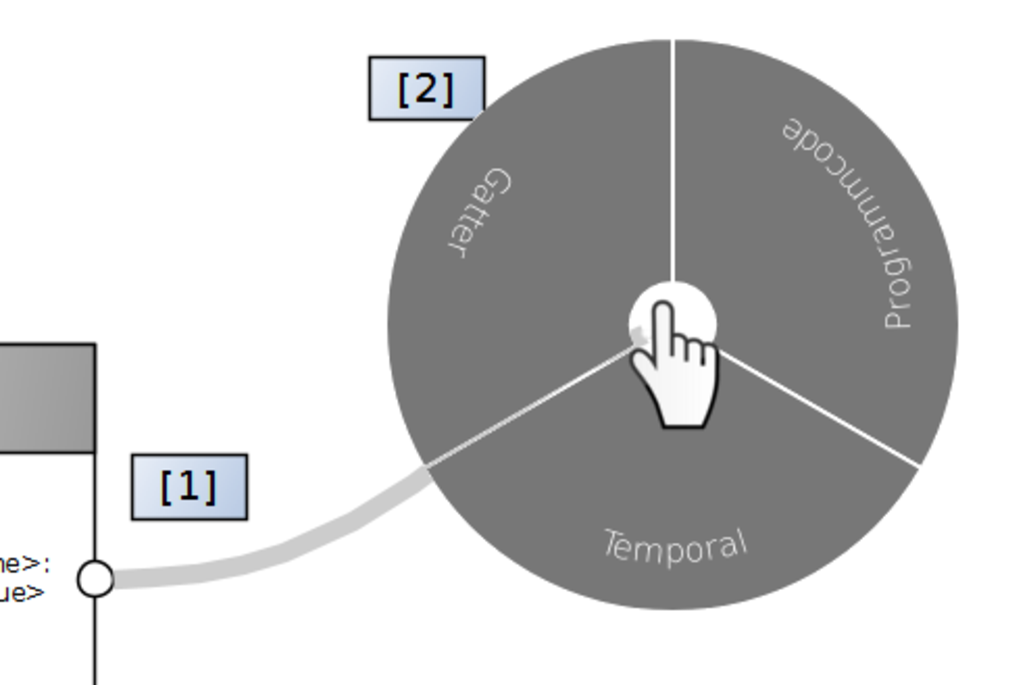
\includegraphics[width=.6\textwidth]{bilder/chapter4/chapter4_3/createNodes.pdf}
  \caption{Das Radialmenu mit den fünf verschiedenen Operationsklassen aus Kapitel \ref{subsubsec:eventtrans} zur Auswahl}
  \label{fig:connectNodesInteraction}
\end{figure}
Die Funktionsknoten sind die einzigen Knoten, die in ihrer Existenz nicht an ein physisches Pendant gebunden sind. Aus diesem Grund, werden sie manuell vom Nutzer erstellt und gelöscht. Die Erstellung von Funktionsknoten geschieht mit Hilfe des Radialmenüs. Ein Funktionsblock kann wie in Abbildung [ref] gezeigt ist auf zwei Weisen erstellt werden: Kontextsensitiv und Kontextunabhängig. \textbf{Kontextunabhängig} können Funktionsknoten auf der ganzen Arbeitsfläche erzeugt werden. Der Benutzer ruft das Radialmenü auf und wählt den gewünschten Knoten aus. \textbf{Kontextsensitiv} ist das Radialmenü Knoten wenn der Endnutzer gerade eine Verbindung erstellt. In diesem Fall, zeigt das Radialmenü nur Optionen an, die für die zu erstellende Verbindung relevant sind. Erstellt der Nutzer bspw. eine Verbindung, die als Quelle den Temperatursensor hat, zeigt das Radialmenü nur Funktionsknoten an, die mit \textit{Number}-Werten (sprich Temperaturwerten) umgehen können. Für den Endnutzer wird der Erstellungsprozess dadurch übersichtlicher, schneller und weniger fehleranfällig.

\subsubsection{Erstellen von \ac{FSM}}\label{FSMkreieren}


\begin{figure}[h]
  \centering
  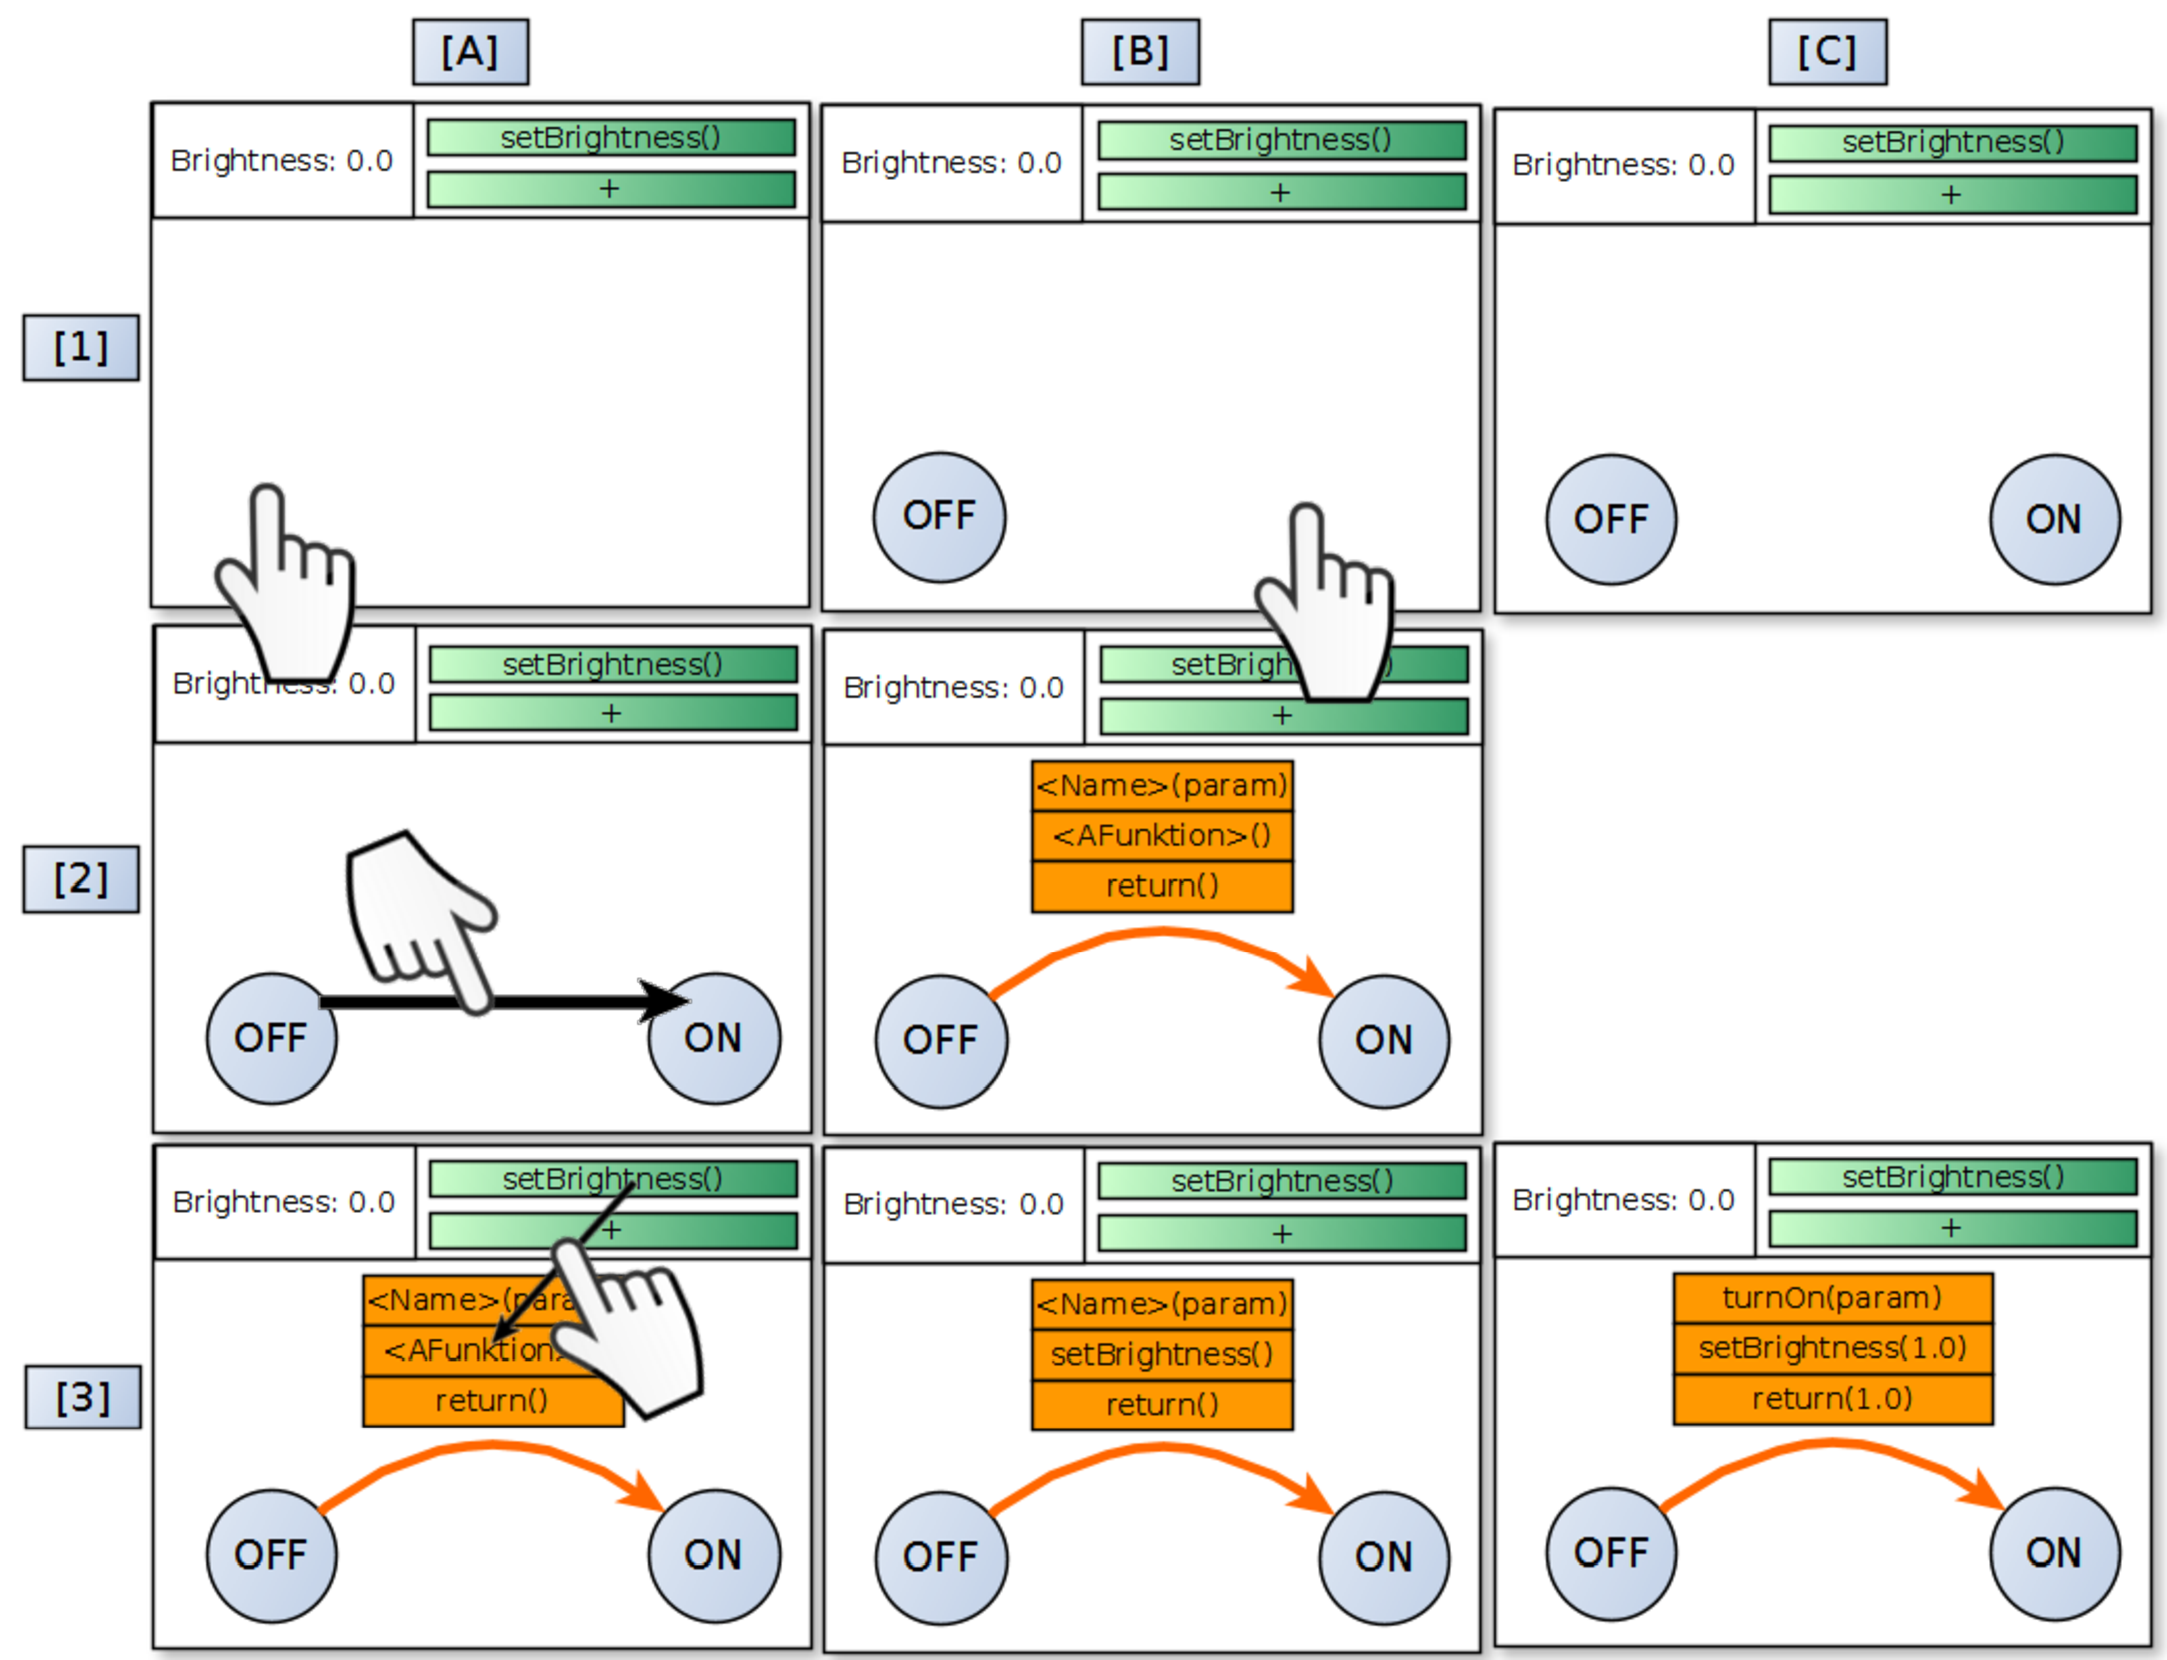
\includegraphics[width=1\textwidth]{bilder/chapter4/chapter4_3/createFsm.pdf}
  \caption{Das Radialmenu mit den fünf verschiedenen Operationsklassen aus Kapitel \ref{subsubsec:eventtrans} zur Auswahl}
  \label{fig:connectNodesInteraction}
\end{figure}

Die \ac{FSM} wird in drei Schritten erstellt:
\begin{enumerate}
    \item Zustände erstellen und benennen
    \item Übergänge ziehen
    \item Übergangslogik definieren
\end{enumerate}
Das Erstellen sämtlicher Komponenten wird hierbei ebenfalls durch \textit{Drag-and-Drop} interaktionen durchgeführt. 

